\chapter{Experiments and Discussions}
For the quantification of how well our system works we need some measurements.
Unfortunately one of our input channels is not functioning (corresponding to the
D string), hence it will be ignored.
To make it simple our measurements will be based on mean and standard deviation.
A few measurements were proposed, as listed:

\begin{itemize}
  \item Single Note Accuracy, \autoref{single-note-accuracy}: by hitting each string
  at a time on only a single note, measurements were taken. The standard deviation line is based on the
  frequency instead of the note, showing how the detected frequency fluctuates around
  the note.
  \item A minor Chord Error, \autoref{am-chord-error}: by hitting all the strings that compose
  the Am chord and comparing the readings with the expected result an error rate (and standard
  deviation) is calculated based on the note (considering cents).
  \item E major Chord Error, \autoref{e-chord-error}: same as above, but for the E major chord.
  \item Chromatic Scale Error, \autoref{chromatic-scale-error}: For each string, a chromatic
  scale was plucked and with the measurements an error rate was calculated. An error is considered
  when two neighbor notes are not integer consecutive values.
  \item Pluck Counting, \autoref{pluck-hits-counting}: by quickly (4 notes/s approximately) hitting
  a string 20 times, the actual number of detected notes are counted.
\end{itemize}

\begin{figure}[!htpb]
  \centering
  \caption{Strings Single Note Accuracy}
  \label{single-note-accuracy}
  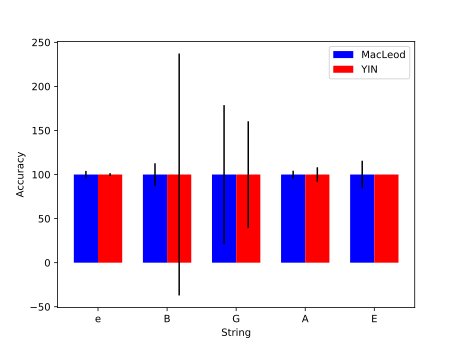
\includegraphics[scale=0.85]{images/measurements/single-note-accuracy}
  \legend{Source: Authors}
\end{figure}

\begin{figure}[!htpb]
  \centering
  \caption{Am Chord Error}
  \label{am-chord-error}
  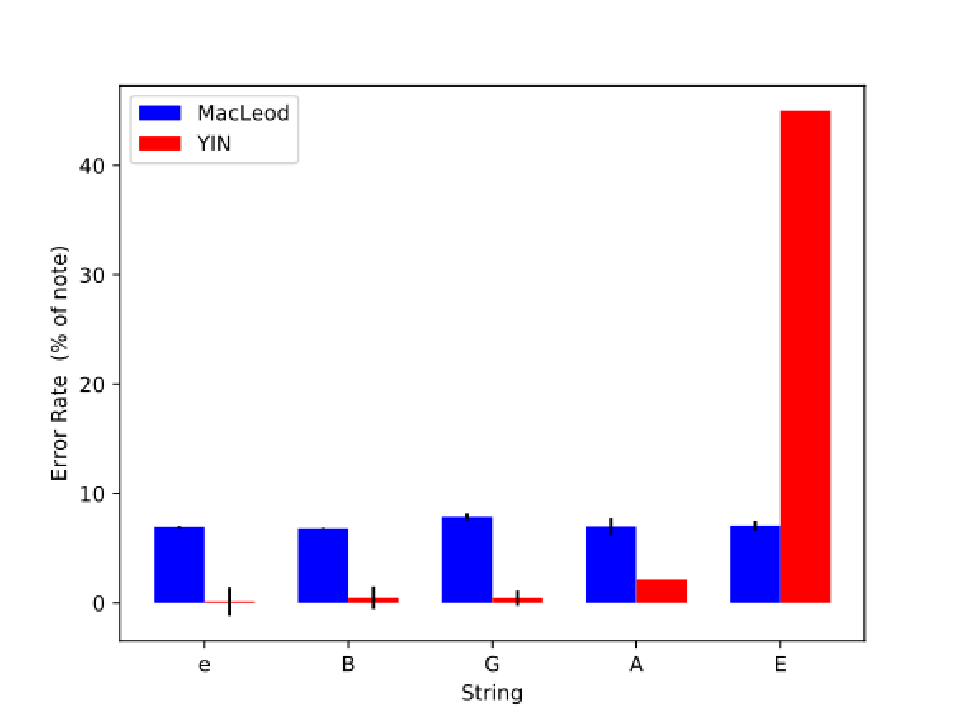
\includegraphics[scale=0.85]{images/measurements/am-chord-error}
  \legend{Source: Authors}
\end{figure}

\begin{figure}[!htpb]
  \centering
  \caption{E Chord Error}
  \label{e-chord-error}
  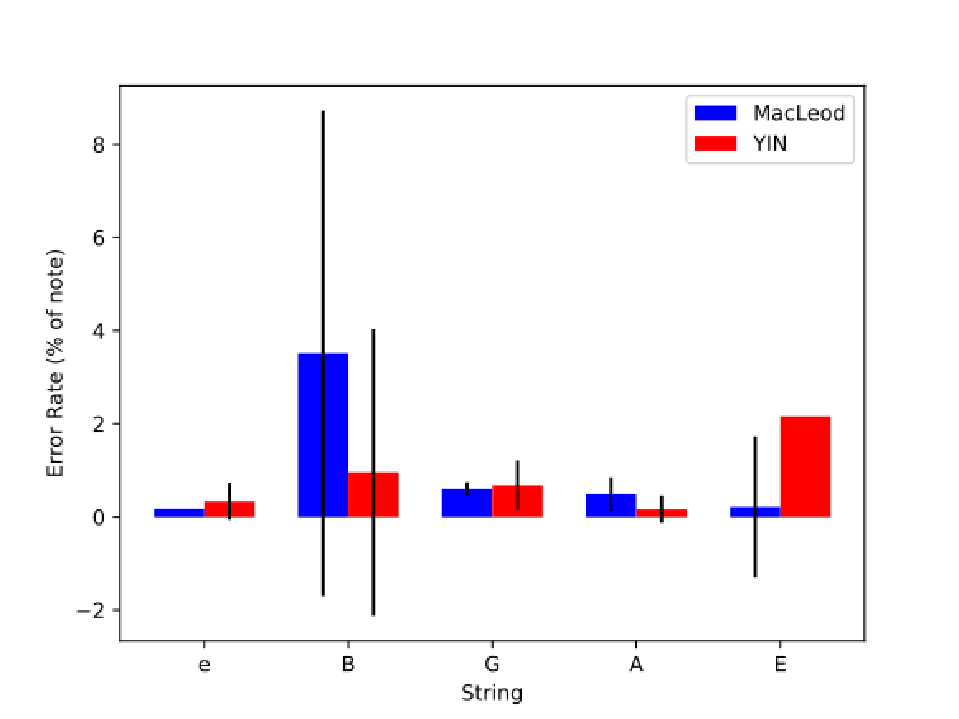
\includegraphics[scale=0.85]{images/measurements/e-chord-error}
  \legend{Source: Authors}
\end{figure}

\begin{figure}[!htpb]
  \centering
  \caption{Chromatic Scale Error}
  \label{chromatic-scale-error}
  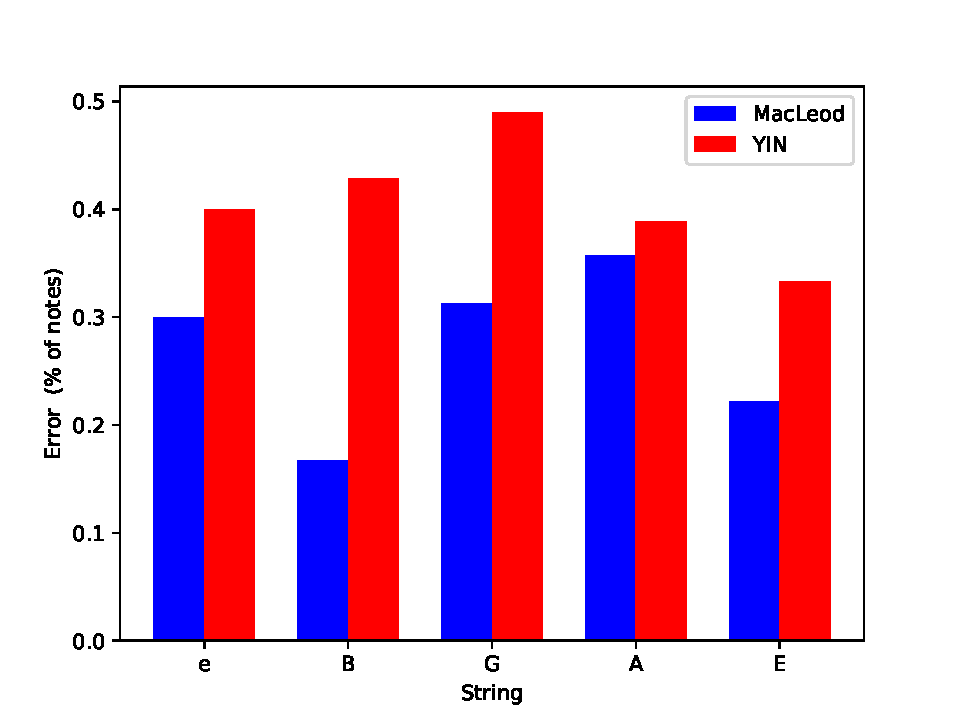
\includegraphics[scale=0.85]{images/measurements/chromatic-scale-error}
  \legend{Source: Authors}
\end{figure}

\begin{table}[htb]
  \begin{center}
    \ABNTEXreducedfont
    \caption[Pluck Hits Counting]{Pluck Hits Counting}
    \label{pluck-hits-counting}
    \begin{tabular}{c|c|c}
      \hline
      Correct Value & MacLeod & YIN \\
      \hline
      20 & 42 & 28 \\
      \hline
    \end{tabular}
    \legend{Source: authors}
  \end{center}
\end{table}

\section{Discussions}
Strings Single Note Accuracy test gave satisfactory results (\autoref{single-note-accuracy}). B string has a high
standard deviation because it's signal has DC noise, due to resistor
imprecisions. This limited the channel gain which ultimately made this
channel results lower than the others. The same analysis is true for
all other experiments.

Both the chord detection experiments (\autoref{am-chord-error}, \autoref{e-chord-error}) gave reasonable results, but they
show our system still has lots of room for improvement. The exception is for
the E string error on the Am chord using the YIN algorithm. The reason
for this is that YIN is not working well for low frequency notes, because
it still needs a greater period (samples) for analysis, which is not currently
possible due to processing time limitations - but a solution is proposed at
the next chapter.

The chromatic scale results (\autoref{chromatic-scale-error}) show that our system is not working well along time.
By using a small period of measurement (so it can run at real-time) the range
where a note is changing to the next one is misread as an incorrect result.
This is a big problem for music annotation, but has the same solution as above,
which needs performance improvement.

The last test (\autoref{pluck-hits-counting}) also shows our time related issues,
that, although being natural, still need to be dealt with, for the same reason above, transitions
through time that need a larger sample period to work well. The reason for the plucking
issue is indeed not given by the amplitude detection, but for frequency variations.
